\documentclass[tikz,border=2pt]{standalone}
\usepackage{pgfplots}
\pgfplotsset{compat=1.18}
\usetikzlibrary{intersections}
\usepgfplotslibrary{fillbetween}

\begin{document}
	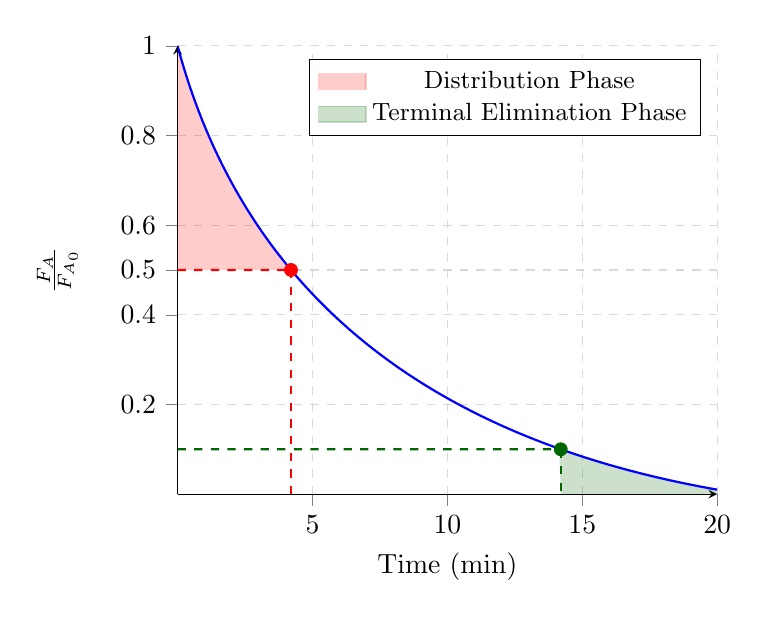
\begin{tikzpicture}
	
	
		\begin{axis}[
			axis lines=middle,
			ymin = 0,
			ymax = 1,
			xmin = 0,
			xmax= 20,
			grid = major,
			grid style={dashed, gray!30},
			ylabel near ticks,
			xlabel near ticks,
			xlabel=Time (min),
			ylabel=$\frac{F_A}{F_{A_0}}$,
			extra y ticks={0.5},
			tick align=outside,
			legend pos= north east,
			legend style={font=\small, cells={align=left}}]
		
		\draw [blue, thick, name path = curve1] (axis cs: 0,1) to[out=285, in=170] (axis cs: 20,0.01);
		\path[name path = line1] (axis cs: 0,0.5)--(axis cs: 5,0.5);

		\draw [red, thick, dashed, name intersections={of=curve1 and line1,by={Int1}}, name path=reddash] (axis cs: 0,0.5) -- (Int1) node[circle,fill=red,inner sep=0pt,minimum size=5pt]{};
		\draw [red, thick, dashed] (Int1) -- +(0,-0.5);

		\path[name path = line2] (axis cs: 0,0.1)--(axis cs: 18,0.1);
		\draw [black!60!green, thick, dashed, name intersections={of=curve1 and line2,by={Int2}}] (axis cs: 0,0.1) -- (Int2) node[circle,fill=black!60!green,inner sep=0pt,minimum size=5pt]{};
		\draw [black!60!green, thick, dashed] (Int2) -- +(0,-0.1);

		\node (root) at (axis cs: 0,0){};
		\path [name path = axis] (Int2 |- root) -- (20,0);

		\addplot [red, opacity = 0.2] fill between [of = curve1 and reddash, soft clip={domain= 0:5}];
		\addplot [black!60!green, opacity = 0.2] fill between [of = curve1 and axis, soft clip={domain=14.15:20}];
		\addlegendentry{Distribution Phase};
		\addlegendentry{Terminal Elimination Phase};


		\end{axis}
	\end{tikzpicture} 
\end{document}